% ============================================================================
%  Attention on Lattice Traversal Is All You Need
%  The EWM Lattice as Map, Attention as Locomotion,
%  and Materialization as the Door Between Them
% ----------------------------------------------------------------------------
%  Build:  pdflatex attention_lattice_traversal.tex   (run twice)
%  notation follows main.tex / companion.tex / tecs_state_machine_trajectory.tex
% ============================================================================
\documentclass[11pt,a4paper]{article}

\usepackage[utf8]{inputenc}
\usepackage[T1]{fontenc}
\usepackage{amsmath,amssymb,amsthm}
\usepackage{amscd}
\usepackage{booktabs}
\usepackage{graphicx}
\usepackage{array}
\usepackage{tikz}
\usetikzlibrary{arrows.meta,positioning,fit,backgrounds,calc}
\usepackage{hyperref}
\usepackage[margin=1in]{geometry}
\usepackage{enumitem}
\usepackage{placeins}
\usepackage{xcolor}
\definecolor{hlblue}{RGB}{0,80,160}
\hypersetup{colorlinks=true,linkcolor=hlblue,urlcolor=hlblue,citecolor=hlblue}

% ---- theorems (aligned with companion.tex / tecs paper) --------------------
\newtheorem{principle}{Principle}[section]
\newtheorem{theorem}[principle]{Theorem}
\newtheorem{definition}[principle]{Definition}
\newtheorem{proposition}[principle]{Proposition}
\newtheorem{corollary}[principle]{Corollary}
\newtheorem{lemma}[principle]{Lemma}
\theoremstyle{remark}
\newtheorem{remark}[principle]{Remark}

% ---- shorthands (aligned with the companion note) --------------------------
\newcommand{\Plane}{\ensuremath{\mathbb{B}}}          % bit plane
\newcommand{\Lat}{\ensuremath{\mathcal{B}}}            % HLLSet (Boolean) lattice
\newcommand{\LatR}{\ensuremath{\mathcal{B}_{\mathbb{R}}}} % realification
\newcommand{\Tok}{\ensuremath{\mathcal{T}}}            % token space
\newcommand{\HLL}{\ensuremath{H}}                      % an HLLSet
\newcommand{\xor}{\ensuremath{\Delta}}                 % ring addition
\newcommand{\Reg}{\ensuremath{\mathsf{M}}}             % register count
\newcommand{\Prec}{\ensuremath{P}}                     % precision
\newcommand{\Bits}{\ensuremath{b}}                     % bits per register
\newcommand{\BSS}{\ensuremath{\mathsf{BSS}}}           % BSS measure
\newcommand{\res}{\ensuremath{\mathrm{res}}}           % residual
\newcommand{\spanof}[1]{\ensuremath{\langle #1\rangle}}% GF(2) span
\newcommand{\Tab}{\ensuremath{\mathsf{T}}}             % a turn
\newcommand{\supp}{\ensuremath{\mathrm{supp}}}         % support
\newcommand{\Attn}{\ensuremath{\mathrm{Attn}}}          % attention operator
\newcommand{\Trv}{\ensuremath{\mathrm{Tr}}}             % traversal operator
\newcommand{\World}{\ensuremath{w}}                     % a world
\newcommand{\Ctx}{\ensuremath{\mathcal{C}}}             % token context
\newcommand{\Img}{\ensuremath{\mathrm{Im}}}             % image
\newcommand{\Lut}{\ensuremath{\mathcal{L}}}             % LUT
\newcommand{\iotaw}{\ensuremath{\iota_{w}}}             % world interpretation
\newcommand{\Bnd}{\ensuremath{\Phi}}                    % bridge
\newcommand{\op}{\ensuremath{\oplus}}                   % OR
\newcommand{\q}{\ensuremath{\mathbf{q}}}                % query vector
\renewcommand{\k}{\ensuremath{\mathbf{k}}}              % key vector (overrides ogonek accent)
\newcommand{\vv}{\ensuremath{\mathbf{v}}}               % value vector
\newcommand{\xx}{\ensuremath{\mathbf{x}}}               % state vector
\newcommand{\sigm}{\ensuremath{\sigma}}                 % score

% ---- title -----------------------------------------------------------------
\title{\textbf{Attention on Lattice Traversal Is All You Need}\\[4pt]
\large The EWM Lattice as Map, Attention as Locomotion,\\
and Materialization as the Door Between Them\\[6pt]
\normalsize Fourth paper in the \textit{Emerging World Models} series}

\author{Alex Mylnikov \and Alexandr Mylnikov Jr. \and Deependra Kumar}
\date{\today}

\begin{document}
\maketitle

\begin{abstract}
Two research programmes have been asking the same question from opposite ends.
Transformer \emph{attention} asks: given a query, which stored items should a
learned, differentiable routing function read, and how much? The \emph{Emerging
World Models} (EWM) lattice asks: given a query \emph{HLLSet}, which
content-addressed nodes of a Boolean lattice should an exact, gradient-free
routing function visit? We argue that the two are neither rivals nor the same
thing: they are the two halves of one journey. \textbf{The lattice is the map}---%
a coarse, exact, persistent, content-addressed graph of places to visit, in
which each node is a compact HLLSet that carries the place's full local detail
in compressed form. \textbf{Attention is the locomotion}---the fine, graduated,
differentiable mechanism that actually moves the model between places once their
detail has been unpacked. \textbf{Materialization is the door}---the morphism
that restores an HLLSet context into a token context the LLM can attend to, and,
by ingestion, re-compresses the result into a new node. The seam between the two
layers is exact and elementary: for nonnegative attention weights, the support
of the attention output is the lattice \emph{join} of the attended value nodes,
so \emph{the bitmap decides which place is in the working set and the weights
decide how the model moves inside it}. The softmax is the entropic (Gibbs)
relaxation of a thresholded selection, so the EWM world threshold is the
attention threshold and temperature is its smooth relaxation. Around the seam
every transformer device has a lattice counterpart: multi-head attention is the
family of \emph{worlds}; the output projection is the \emph{bridge}; depth is
complement traversal with the Noether stop; causal masking is the \emph{monotone
ring basis}; the KV cache is the \emph{commit DAG}; the residual stream is the
\emph{union invariant} and the $D/R/N$ decomposition; and Q/K/V projections are
the \emph{bootstrap permutation} that closes Ashby's variety gap. The result is
a win-win integration: the lattice gives the model a durable, exact, auditable
map and a context it can shrink and expand at will; attention gives the lattice
a differentiable way to travel, resolve collision detail, and generate the next
node. We prove the support--union lemma and the correspondence theorem, state
the structural dictionary, describe the travel loop and the exact engine's three
modes, and restate ``all you need'' precisely: attention \emph{on} lattice
traversal---the map, the motion, and the door---is the complete primitive.
\end{abstract}

\noindent\textbf{Keywords:} attention; world models; HLLSet; Boolean lattice;
content addressing; softmax; traversal; materialization; context management;
KV cache; residual stream; IICA.

% ============================================================================
\section{Introduction}
\label{sec:intro}
% ============================================================================

Transformer attention \cite{vaswani2017} is, mechanically, one line:
\[
  \Attn(X) \;=\; \mathrm{softmax}\!\left(\frac{QK^{\top}}{\sqrt{d}}\right) V,
  \qquad Q=XW_Q,\quad K=XW_K,\quad V=XW_V .
\]
Everything that follows in a modern language model---multi-head splits,
causal masks, residual streams, KV caches, flash-attention kernels---is a
variation on how that one line is organised, computed, or fed. The line has
been read as retrieval \cite{lewis2020}, as associative memory
\cite{ramsauer2020}, as kernel smoothing \cite{choromanski2021}, and as
hashing \cite{kitaev2020}. What all of these readings share is that attention
is \emph{content-based routing followed by a monotone accumulation}: a query
selects items by a similarity and their values are combined.

The \emph{Emerging World Models} (EWM) programme \cite{ewm2026,companion2026}
arrives at the same shape from the opposite direction. Its state is a
content-addressed set---an \textbf{HLLSet}, a compact bit-vector sketch of a
token collection over a fixed $32$K-bit plane---whose subsets form a Boolean
lattice $\Lat$. The state machine built on this lattice \cite{state2026} turns
a query into a traversal: a query HLLSet is ingested, a set of stored HLLSet
nodes is scored by a symmetric, content-addressed similarity (overlap,
containment, BSS), the selected nodes are accumulated by \emph{join} (union),
and the result is materialised back to tokens.

The two are close, and the closeness is real---but it is not an identity, and it
is not a competition. This paper argues that they are the two halves of one
journey.

\paragraph{The traveller's analogy.}
Before a journey, one consults a \emph{map}. The map names the places worth
visiting and how they connect, but it is deliberately coarse: it does not tell
you how to board the train. EWM's lattice is that map---a coarse, exact,
persistent, content-addressed graph of nodes, each a compact HLLSet. The detail
lives \emph{inside} the node: the transportation, the ticket, the hotel are all
there, but compressed. The bitmap is the coordinate, not the itinerary. To
actually \emph{move} from one place to the next, the traveller must unpack the
node's detail and act on it; in our terms, the node is \textbf{materialised}
into a token context, and the LLM's graduated attention does the moving. The two
layers are therefore complementary rather than identical: the lattice answers
\emph{which place}, and attention answers \emph{how to travel once there}.

\paragraph{Thesis.}
\emph{Attention is the locomotion that runs on the EWM lattice's map; the
lattice is the exact navigation layer that attention lacks, and attention is the
differentiable navigation the lattice cannot provide on its own.} The seam
between the two layers is a single exact operator: for nonnegative attention
weights, the support of the attention output is the lattice join of the attended
value nodes, so the \emph{bitmap} fixes the working set and the \emph{weights}
move within it. Materialisation is the door that restores HLLSet context to
token context; ingestion is the same door the other way. The integration is a
win-win: neither layer subsumes the other, and together they close the travel
loop.

\paragraph{Contributions.}
\begin{enumerate}[leftmargin=*,nosep]
  \item \textbf{The support--union lemma (\S\ref{sec:bridge}).} For Boolean
    value nodes $V_i$ and nonnegative attention weights $\alpha_i$, the support
    of the attention output is the bitwise join of the attended nodes:
    $\supp(\sum_i \alpha_i V_i)=\bigcup_{i:\alpha_i>0}V_i$. Hence an attention
    layer's \emph{bitmap} is a node of the EWM lattice, and the weights live one
    level up, in its realification. This is the exact seam between the map and
    the motion.
  \item \textbf{The correspondence theorem (\S\ref{sec:bridge}).} A truncated
    scaled-dot-product attention head is the unique free-energy minimiser of a
    traversal score, and its support is the $\theta$-thresholded traversal
    join. The two layers share one support operator and one similarity geometry;
    they differ only in the convex interpolation inside the support.
  \item \textbf{The travel loop and the door (\S\ref{sec:map}).} We formalise
    the node as a place with compressed detail, materialization as the door that
    unpacks it into token context (with the round-trip composition law as the
    door's fidelity guarantee), and context management as lattice shrink/expand
    before materialisation. This is the practical win-win.
  \item \textbf{The structural dictionary (\S\ref{sec:dictionary}).} Heads are
    worlds; the output projection is the bridge; depth is complement traversal
    with the Noether stop; causal masking is the monotone ring basis; positions
    are rotating coordinates; the KV cache is the commit DAG; the residual
    stream is the union invariant and $D/R/N$; Q/K/V projections are the
    bootstrap permutation.
  \item \textbf{The exact engine (\S\ref{sec:engine}).} The three modes---%
    address-key, set-key, and hybrid---form a spectrum from the fully learned
    relaxation to the exact content-addressed traversal, with the coverage
    invariant as the exactness gauge.
  \item \textbf{A precise reading of ``all you need'' (\S\ref{sec:all}).} The
    complete primitive is the pair: the map has no motor, the motor has no map,
    and the door is what lets one hand work to the other.
\end{enumerate}

\paragraph{Roadmap.} Section~\ref{sec:attn} recalls attention.
Section~\ref{sec:ewm-bg} recalls the EWM lattice, opening with a one-page
HLLSet primer (\S\ref{sec:primer}) for readers new to the construction.
Section~\ref{sec:bridge}
proves the seam. Section~\ref{sec:map} develops the map-and-journey integration.
Section~\ref{sec:dictionary} states the structural dictionary.
Section~\ref{sec:engine} describes the exact engine.
Section~\ref{sec:all} restates the thesis and its limits;
Sections~\ref{sec:related}--\ref{sec:conclusion} place it and close.

\begin{remark}[The Glass Bead Game]
Hesse's \emph{Glass Bead Game} \cite{hess1943} is played by threading beads
drawn from every discipline into one formal language; the player's skill is the
move that makes the whole board legible. This paper is one move. The beads are
the objects of the EWM corpus---HLLSets, worlds, the ring, the trajectory, the
bridge; the board is the map; and the observation is that the lattice has been
drawing the map, attention has been walking it, and materialization has been the
door between them all along.
\end{remark}

% ============================================================================
\section{Attention, recalled}
\label{sec:attn}
% ============================================================================

Let $X\in\mathbb{R}^{n\times d}$ be a sequence of $n$ token states. A single
head computes
\begin{equation}
\label{eq:attn}
Q=XW_Q,\quad K=XW_K,\quad V=XW_V,\qquad
A=\mathrm{softmax}\!\left(\frac{QK^{\top}}{\sqrt d}\right),\qquad
\Attn(X)=AV,
\end{equation}
with $W_Q,W_K,W_V\in\mathbb{R}^{d\times d_k}$, $A\in\mathbb{R}^{n\times n}$ row-
stochastic, and the softmax applied row-wise. Five features make this the
mechanism that matters.

\begin{enumerate}[leftmargin=*,nosep]
  \item \textbf{Content routing.} The score $\sigm_{ij}=\q_i\!\cdot\!\k_j$ is a
    function of the two states alone. Order enters only through the position
    encoding and the mask; the routing itself is order-free.
  \item \textbf{Permutation equivariance.} Permuting the tokens permutes the
    rows and columns of $A$ and the rows of $\Attn(X)$ identically. Attention
    cannot tell two orderings apart unless a position signal is added.
  \item \textbf{Competition.} The row-wise softmax normalises the scores, so
    keys compete for a fixed unit of weight. This is the selection step.
  \item \textbf{Value aggregation.} The output is a convex combination of the
    values, $\Attn(X)_i=\sum_j A_{ij}\vv_j$.
  \item \textbf{Composability.} Heads are concatenated and projected by $W_O$,
    and blocks are stacked around a residual stream
    $\xx_{l+1}=\xx_l+\mathrm{MHA}_l(\xx_l)$ with a normalisation and a
    feed-forward network.
\end{enumerate}

Two structural remarks are used later. First, the score is invariant under
$Q\mapsto QA$, $K\mapsto KA^{-\top}$ for any invertible $A$
\cite{cortex2026}; the only invariant object is the matrix of pairwise
similarities, and the labelled ontology attached to $K$ is an interpretation,
not part of the mechanism. Second, because softmax is strictly positive, a
plain attention row has \emph{no zeros}: $A_{ij}>0$ for every pair. Selection
in attention is therefore never hard; it is a matter of degree, and any
hard retrieval must be imposed by a threshold or a sparsity mask. Both remarks
reappear as the two axes of the seam: \emph{similarity} and
\emph{threshold}.

% ============================================================================
\section{The EWM lattice, recalled}
\label{sec:ewm-bg}
% ============================================================================

We keep this section to the minimum needed for the seam; the full development
is in the main EWM paper \cite{ewm2026}, the lattice/world companion
\cite{companion2026}, and the state-machine paper \cite{state2026}.

\paragraph{A primer first.} Section~\ref{sec:primer} gives a one-page
introduction to HLLSets for readers meeting the construction for the first
time; the rest of the section recaps the corpus's notation.

\subsection{A short introduction to HLLSets}
\label{sec:primer}

An \textbf{HLLSet} is a compact, fixed-size \emph{sketch} of a collection of
items---here, tokens. Instead of storing the items, it stores a bit-vector whose
set bits mark the positions the items hashed into. A collection of ten tokens
and a collection of ten million become the same kind of object: $32{,}768$ bits,
or $4$\,KB packed. The sketching idea is borrowed from Bloom filters and
HyperLogLog \cite{bloom1970,flajolet2007}---a set represented by a fixed-size
pattern of hash-derived positions---but EWM uses it differently: the sketch is
not a cardinality estimator, it is the \emph{state}, and all sketches share one
plane, so set operations on them are exact bit operations.

\paragraph{How one is built, in one breath.} Fix the geometry once. Precision
$\Prec$ gives $\Reg=2^{\Prec}$ registers of $\Bits$ bits each, so the
\textbf{bit plane} $\Plane=\{0,\dots,\Reg\cdot\Bits-1\}$ has $32{,}768$
positions at the defaults $\Prec=10$, $\Bits=32$. Then, for each item $t$:
\begin{enumerate}[leftmargin=*,nosep]
  \item hash it once, $h(t)$;
  \item split the hash into a register index and a trailing-zero state,
    \begin{equation}
    \label{eq:position}
    \mathrm{reg}(t)=h(t)\bmod \Reg,\qquad
    \mathrm{tz}(t)=\mathrm{clamp}\bigl(\mathrm{trailing\_zeros}(h(t)\gg\Prec),\,0,\,\Bits-1\bigr),
    \end{equation}
    naming a single \textbf{bit address}
    $\mathrm{bit}(t)=\mathrm{reg}(t)\cdot\Bits+\mathrm{tz}(t)$;
  \item set that bit---OR it into the sketch.
\end{enumerate}
Nothing else happens. Order does not matter (OR is commutative) and repetition
does not matter (OR is idempotent). A side index, the \textbf{LUT}, records for
each bit which items hashed there, so the process can be read back.

\paragraph{Illustration.} Suppose three tokens land as follows (Figure~\ref{fig:hllset};
addresses chosen for the picture, on a toy plane of sixteen positions rather
than $32{,}768$):
\texttt{cat}$\to3$, \texttt{sat}$\to9$, \texttt{mat}$\to3$. Then
$\HLL(\{\texttt{cat},\texttt{sat}\})=\{3,9\}$ and
$\HLL(\{\texttt{mat}\})=\{3\}$; the union is $\{3,9\}$, the meet is $\{3\}$, and
the LUT reads bit~$3$ back as $\{\texttt{cat},\texttt{mat}\}$. Two different
tokens can share a bit---a \emph{collision}---which is why the LUT, not the
bitmask, carries the meaning.

\begin{figure}[t]
\centering
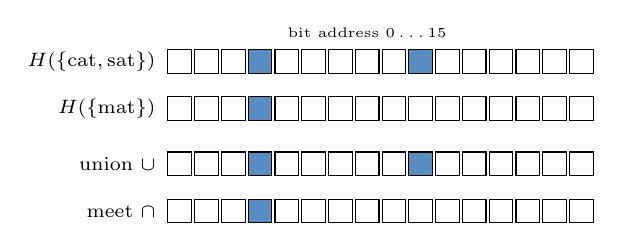
\begin{tikzpicture}[font=\scriptsize, inner sep=0pt,
  bit/.style={draw, minimum size=0.30cm, inner sep=0pt},
  on/.style={bit, fill=hlblue!65}]
\foreach \c in {0,...,15}{\node[bit] at (\c*0.34,0) {};}
\node[on] at (3*0.34,0) {}; \node[on] at (9*0.34,0) {};
\node[anchor=east,font=\scriptsize] at (-0.30,0) {$\HLL(\{\mathrm{cat},\mathrm{sat}\})$};
\foreach \c in {0,...,15}{\node[bit] at (\c*0.34,-0.6) {};}
\node[on] at (3*0.34,-0.6) {};
\node[anchor=east,font=\scriptsize] at (-0.30,-0.6) {$\HLL(\{\mathrm{mat}\})$};
\foreach \c in {0,...,15}{\node[bit] at (\c*0.34,-1.3) {};}
\node[on] at (3*0.34,-1.3) {}; \node[on] at (9*0.34,-1.3) {};
\node[anchor=east,font=\scriptsize] at (-0.30,-1.3) {union $\cup$};
\foreach \c in {0,...,15}{\node[bit] at (\c*0.34,-1.9) {};}
\node[on] at (3*0.34,-1.9) {};
\node[anchor=east,font=\scriptsize] at (-0.30,-1.9) {meet $\cap$};
\node[anchor=south,font=\tiny] at (7*0.34,0.30) {bit address $0\dots15$};
\end{tikzpicture}
\caption{A toy HLLSet plane (sixteen positions, for the picture only). The top
two rows sketch two token collections, the bottom two their join and meet. Set
operations are bitwise and exact; position~$3$ is shared because \texttt{cat}
and \texttt{mat} collide there, and the LUT---not the bits---records which token
is which.}
\label{fig:hllset}
\end{figure}

\paragraph{What it buys.} Three properties are used throughout this paper.
\emph{Fixed size}: a waypoint is always $4$\,KB, so a model can hold a great
many of them---this is what makes the lattice a usable map. \emph{Exact set
algebra}: union, intersection, difference, and symmetric difference are bitwise
and exact on the shared plane, and two sketches are compared by their overlap
(Lemma~\ref{lem:overlap}). \emph{Monotone, content-addressed accumulation}:
union is idempotent, commutative, and associative, so independent contributions
merge without coordination, and the SHA-1 digest of the bits is the sketch's
name. The one price is collisions, and they are managed by the LUT and by
re-hashing under further seeds (\S\ref{sec:engine}).

\paragraph{From the sketch to the lattice.} Write
$\HLL(A)=\bigcup_{t\in A}\{\mathrm{bit}(t)\}$ for the sketch of a token
collection $A\subseteq\Tok$. Because every HLLSet is a subset of the one common
plane, sketches are automatically a lattice under inclusion:
\begin{equation}
\label{eq:lattice}
\Lat=\bigl(2^{\Plane},\ \subseteq,\ \cup,\ \cap,\ \xor\bigr),
\end{equation}
with join $\cup$ (bitwise OR), meet $\cap$ (AND), and ring addition $\xor$
(symmetric difference). $2^{\Plane}$ is a Boolean lattice; equivalently, if we
read a bit-vector as a $\{0,1\}$ vector, $\Lat$ is the vertex set of the
$32$K-dimensional hypercube. This lattice is the map the rest of the paper
traverses.

\paragraph{IICA morphisms.} The token-to-node connection is a chosen
\textbf{measurement morphism} $\mu:\{\text{token collections}\}\to\Lat$. The
model requires only that $\mu$ be \textbf{IICA}: \emph{Idempotent} (the same
collection always yields the same bits), \emph{Immutable} (bits are never
mutated; only new nodes appear), and \emph{Content-Addressed} (a node is named
by a digest of its content). Any algorithm satisfying IICA is interchangeable;
the SHA-1 digest of an HLLSet is its identity, and ``existence is registration''
\cite{companion2026}. Two instances matter here: the \emph{flat projection}
$\mu_{\mathrm{flat}}$, which is a join homomorphism
$\mu_{\mathrm{flat}}(A\cup B)=\mu_{\mathrm{flat}}(A)\cup\mu_{\mathrm{flat}}(B)$,
and \emph{windowed $n$-gram ingestion} $\mu_{ng}$, which is
inclusion-isotonic but not a join homomorphism.

\paragraph{Worlds.} The hash function enters as a parameter of the
measurement, not of the lattice. Write $\World=(h,s,\tau)$ for a hash
configuration $(h,s)$---hash type and seed---together with a BSS threshold
$\tau$. A world induces a measurement $\mu_\World:2^{\Tok}\to\Lat$, a
thresholded node set
\begin{equation}
\label{eq:world}
\mathcal{N}_\tau(\World)=\bigl\{X\in\Lat_\World:\BSS_\World(X)\ge\tau\bigr\},
\qquad
\BSS_\World(X)=\frac{|X\cap B_\World|}{|B_\World|},
\end{equation}
and an \emph{interpretation} $\iotaw:\Lat\to2^{\Tok}$ that reads a node's bits
back through the world's LUT $\Lut_\World$. Worlds share the representation
plane and separate only in their interpretation
\cite{companion2026}; two worlds communicate only through the \textbf{bridge}
\begin{equation}
\label{eq:bridge}
\Bnd_{\World_1\to\World_2}
=\mathrm{ingest}_{\World_2}\circ\mathrm{transcribe}\circ\mathrm{materialize}_{\World_1},
\end{equation}
which is deterministic, idempotent on builders, and monotone, and which carries
\emph{encodings, not content}.

\paragraph{Traversal and the state machine.} The EWM roles of the three
attention objects are already written down in the cortex design notes
\cite{kspace2026}: $Q=I(\text{query})$ is a fresh ingestion of the query into
the lattice; $K$ is the stored context sub-lattice, content-addressed by CID;
$V=M(K\cap Q)$ is the materialised tokens of the matched subset; and the score
is a lattice morphism---BSS containment, Jaccard, or overlap popcount. The
state machine \cite{state2026} advances a state by
\begin{equation}
\label{eq:fundamental}
H(t)=\bigl(S(t),\,H(t{-}1),\,D,\,R,\,N\bigr),
\end{equation}
where $S(t)$ is the emerging working state, $H(t{-}1)$ the committed base, and
\begin{equation}
\label{eq:drn}
N=S(t)\setminus H(t{-}1),\qquad
R=S(t)\cap H(t{-}1),\qquad
D=H(t{-}1)\setminus S(t)
\end{equation}
are the new, retained, and departed parts. The ring keeps a \emph{monotone
basis} of the span of the committed originals; the span only grows, coordinates
transport exactly across commits by a change-of-basis matrix, and one turn is
the six-step transformation \emph{encode, ingest, join, ring-push, commit,
materialise} \cite{state2026}. The context design \cite{ctx2026} adds the piece
this paper needs most: a conversation is itself an HLLSet, and
\emph{materialize-to-prompt} turns that HLLSet context into a conventional LLM
prompt.

% ============================================================================
\section{The seam: where attention and traversal meet}
\label{sec:bridge}
% ============================================================================

\subsection{Traversal}

\begin{definition}[Traversal]
\label{def:traversal}
Let $\Lat$ be the EWM lattice and let $\LatR=\mathbb{R}^{\Plane}$ be its
\emph{realification}, with $\Lat\hookrightarrow\LatR$ the inclusion of a
bit-vector as a $\{0,1\}$ vector. A \textbf{traversal} of a keyed set
$\mathcal{K}=\{(K_i,V_i)\}_{i=1}^{n}\subseteq\Lat\times\Lat$ by a query
$Q\in\Lat$ with score $\sigm:\Lat\times\Lat\to\mathbb{R}$ consists of a
\emph{selection} and an \emph{accumulation}:
\[
  \text{select:}\quad i\in S \iff \sigm(Q,K_i)\ \text{passes a rule},
  \qquad
  \text{accumulate:}\quad R=\textstyle\bigcup_{i\in S}V_i .
\]
The \textbf{soft traversal} readout at temperature $\tau>0$ replaces the hard
selection by the convex aggregation
\begin{equation}
\label{eq:soft}
R^{(\tau)}(Q)=\sum_{i=1}^{n}\alpha_i(\tau)\,V_i,
\qquad
\alpha_i(\tau)=\frac{e^{\sigm(Q,K_i)/\tau}}{\sum_{j}e^{\sigm(Q,K_j)/\tau}},
\end{equation}
and the \textbf{thresholded traversal} readout at level $\theta$ replaces it by
\begin{equation}
\label{eq:hard}
\Trv_\theta(Q)=\bigcup_{i:\,\sigm(Q,K_i)\ge\theta} V_i .
\end{equation}
A traversal is \textbf{lattice-compatible} when $\sigm$ factors through the
overlap form (\S\ref{sec:overlap}) and the accumulation is the lattice join.
\end{definition}

Comparing \eqref{eq:soft}--\eqref{eq:hard} with \eqref{eq:attn} is already most
of the seam: identify $Q$ with a query vector, $K_i$ with a stored key
vector, $V_i$ with a value vector, and $\sigm$ with the dot product. The only
difference is that Definition~\ref{def:traversal} permits a \emph{hard}
selection, which attention hides inside the softmax. The next two lemmas make
the seam exact.

\subsection{The overlap form}
\label{sec:overlap}

\begin{lemma}[Overlap is a bilinear form]
\label{lem:overlap}
Identify a bit-vector $X\subseteq\Plane$ with its indicator
$x\in\{0,1\}^{\Plane}\subset\mathbb{R}^{\Plane}$. Then for all $X,Y\subseteq\Plane$,
\begin{equation}
  \langle x,y\rangle \;=\;\sum_{b\in\Plane}x_by_b \;=\;|X\cap Y| ,
\end{equation}
so the lattice meet is the multiplication of the inner product on $\LatR$.
Moreover the similarity measures used by EWM are functions of this form:
\[
  \BSS_Y(X)=\frac{\langle x,y\rangle}{|Y|},
  \qquad
  \mathrm{Jaccard}(X,Y)=\frac{\langle x,y\rangle}{|X|+|Y|-\langle x,y\rangle},
  \qquad
  \mathrm{contain}(X,Y)=\frac{\langle x,y\rangle}{|Y|}.
\]
\end{lemma}

\begin{proof}
Both sides count the coordinates $b$ with $x_b=y_b=1$, i.e.\ the bits in
$X\cap Y$; the three displayed identities are immediate from that count.
\end{proof}

Lemma~\ref{lem:overlap} is the reason a lattice traversal is a geometry and not
merely a set operation. The Boolean lattice embedded in $\LatR$ carries the
standard inner product, and its meet is a bilinear pairing; the similarity
measures EWM uses are the normalised pairings. A learned transformer score
$\q_i\!\cdot\!\k_j$ is therefore not a foreign object imposed on the lattice:
it is the same bilinear form after a learned change of basis and a learned
diagonal metric, i.e.\ after the linear maps $W_Q,W_K$. The projections are a
\emph{re-coordinatisation} of the overlap form; the form itself is intrinsic.
This is why the map and the motion can be joined at all: the lattice's notion of
``near'' and attention's notion of ``similar'' are the same form.

\subsection{The support of attention is a lattice join}

\begin{lemma}[Support--union]
\label{lem:support}
Let $V_1,\dots,V_n\in\{0,1\}^{\Plane}\subset\mathbb{R}^{\Plane}$ be Boolean
value nodes and let $\alpha_i\ge 0$. Then
\begin{equation}
  \supp\!\left(\sum_{i=1}^{n}\alpha_i V_i\right)
  \;=\;\bigcup_{i:\,\alpha_i>0} V_i ,
\end{equation}
where $\supp$ is the set of coordinates with a non-zero entry and the union is
bitwise OR. In particular, for the truncated weights
$\alpha_i=\alpha_i(\tau)\cdot\mathbf{1}[\sigm(Q,K_i)\ge\theta]$,
\[
  \supp\bigl(R^{(\tau,\theta)}(Q)\bigr)=\Trv_\theta(Q).
\]
\end{lemma}

\begin{proof}
The left-hand side contains $b$ iff $\sum_i\alpha_i V_{i,b}>0$. Because every
$\alpha_i\ge0$ and $V_{i,b}\in\{0,1\}$, the sum is positive iff some $i$ with
$\alpha_i>0$ has $V_{i,b}=1$, i.e.\ iff $b\in\bigcup_{\alpha_i>0}V_i$. The
truncated statement is the same computation after zeroing the sub-threshold
weights.
\end{proof}

Lemma~\ref{lem:support} is the heart of the paper. Read with
Definition~\ref{def:traversal} it says:

\begin{quote}
\emph{The support of an attention layer is exactly a traversal join: the layer's
bitmap is a node of the EWM lattice. The attention weights never change which
bits are kept---they only decide the convex coordinates inside the kept
support. The bitmap decides which place is in the working set; the weights
decide how the model moves inside it.}
\end{quote}

Two consequences are worth separating. First, because all weights are
nonnegative, attention cannot cancel support: it can only \emph{add} bits, and
the accumulated bitmap is monotone in the set of attended keys. This is the
lattice's monotone join appearing inside the transformer. Second, the weights
are where attention's arithmetic lives, and the support is where its
\emph{state} lives; the two levels---realification and lattice---are exactly
the two levels EWM's companion note distinguishes (shared representation,
separate reading) \cite{companion2026}. Attention is the map that carries the
soft level back down to the lattice level by support---which is precisely what
the door of \S\ref{sec:map} does operationally.

\subsection{Temperature is the entropic relaxation of the threshold}

\begin{theorem}[Free-energy characterisation]
\label{thm:free}
Fix scores $s_i=\sigm(Q,K_i)$ and a temperature $\tau>0$. On the simplex
$\Delta=\{\alpha\in\mathbb{R}^n_{\ge0}:\sum_i\alpha_i=1\}$ the softmax
\eqref{eq:soft} is the unique minimiser of the free energy
\begin{equation}
\label{eq:free}
  F_\tau(\alpha)=-\langle\alpha,s\rangle+\tau\!\sum_{i=1}^{n}\alpha_i\ln\alpha_i ,
\end{equation}
and the minimiser over the sub-simplex supported on $\{i:s_i\ge\theta\}$ is the
truncated softmax. Consequently
\[
  \lim_{\tau\to0^+}\alpha_i(\tau)=
  \begin{cases}1/|M|,& i\in M=\arg\max_j s_j,\\ 0,&\text{otherwise,}\end{cases}
  \qquad
  \lim_{\tau\to\infty}\alpha_i(\tau)=\tfrac1n ,
\]
and the support at any $\tau$ is the $\theta$-superlevel set
$\{i:s_i\ge\theta\}$.
\end{theorem}

\begin{proof}
The Lagrangian of \eqref{eq:free} with the multiplier $\lambda$ for
$\sum\alpha_i=1$ is $-s_i+\tau(\ln\alpha_i+1)-\lambda=0$, giving
$\alpha_i\propto e^{s_i/\tau}$; the truncated version follows by restricting the
simplex. The limits are the standard low- and high-temperature limits of the
Gibbs distribution; the support statement is the definition of the restricted
simplex.
\end{proof}

Theorem~\ref{thm:free} identifies the two knobs precisely. The EWM world
threshold $\tau$ of \eqref{eq:world} is the attention threshold $\theta$: it is
the \emph{hard} (zero-temperature) selection rule. The transformer's softmax
temperature is the \emph{entropic} relaxation of that rule---the device that
makes the hard superlevel set differentiable by allowing every key a small
weight. ``Attention'' and ``traversal'' are therefore not two algorithms with a
resemblance; they are the two ends of one temperature axis, and the softmax is
the annealing schedule between them.

\subsection{The correspondence theorem}

\begin{theorem}[Attention--traversal correspondence]
\label{thm:correspondence}
Let $\mathcal{K}=\{(K_i,V_i)\}$ be a keyed set of Boolean lattice nodes, let
$\sigm$ factor through the overlap form, and fix $\tau>0$ and $\theta$. Then
scaled-dot-product attention \eqref{eq:attn} with truncated softmax at
$\theta$ and traversal \eqref{eq:hard} satisfy:
\begin{enumerate}[leftmargin=*,nosep]
  \item \emph{(support)} $\supp(\Attn_\theta(Q))=\Trv_\theta(Q)$;
  \item \emph{(weights)} the attention row is the unique free-energy minimiser
    on the $\theta$-supported simplex;
  \item \emph{(limits)} as $\tau\to0$ the attention output tends to the value
    average over the argmax set and $\Trv_\theta$ to the join of the argmax
    set; as $\tau\to\infty$ both keep the same support and the output tends to
    the uniform average within it;
  \item \emph{(equivariance)} both operators are equivariant under a
    simultaneous permutation of the keys: $\sigm$ and the join are
    order-independent.
\end{enumerate}
Hence attention and lattice traversal share one support operator, one
similarity geometry, and one accumulation law; they differ only in the convex
interpolation inside the support.
\end{theorem}

\begin{proof}
(1) is Lemma~\ref{lem:support}; (2) is Theorem~\ref{thm:free}; (3) combines the
limits of Theorem~\ref{thm:free} with the fact that the join over a shrinking
support converges to the join over the limiting support (finite unions commute
with limits of finite indicator families); (4) is immediate because
$\sigm(Q,K_i)$ depends on $K_i$ alone and $\cup$ is commutative, so relabelling
the keys relabels the scores without changing the support or the join.
\end{proof}

The theorem describes the \emph{seam}, not a merger. It says that where the two
layers meet---at the support of a selection---they agree on one operator, so a
traversal's output can be handed to an attention layer without translation
loss, and an attention layer's output can be handed back to the lattice as a
node. It does \emph{not} say that the layers do the same job: the traversal
decides \emph{which} nodes are in play and maintains them exactly, while
attention decides \emph{how} to move within the detail those nodes carry. The
next section makes the division of labour explicit.

% ============================================================================
\section{The map and the journey: materialization as the door}
\label{sec:map}
% ============================================================================

The correspondence theorem is the seam. But the two layers do different jobs,
and stating the division of labour explicitly is the paper's practical claim.

\subsection{The node is a place with its detail compressed inside}

An HLLSet is a \emph{coordinate}, not a transcript. The node a traversal selects
is a fixed $32$K-bit sketch; everything the place contains---lexical detail,
structural order, co-occurrence, local statistics---is either folded into those
bits or carried alongside them in the world's LUT and adjacency matrix
\cite{ctx2026}. This is what makes the map cheap: the traveller can hold a great
many destinations at once, because each is a node, and nodes are addressed and
compared by content. The detail is not lost; it is \emph{compressed}, waiting
behind the door.

\subsection{Materialization is the door}

To act inside a node, the model needs the detail in a form it can compute on:
tokens and their embeddings. \textbf{Materialization} is the morphism that
restores an HLLSet context into a token context---the
\emph{materialize-to-prompt} step of the context design \cite{ctx2026}:
\begin{equation}
\label{eq:door}
\Ctx_{\mathrm{tok}}
\ \xrightarrow{\ \mathrm{ingest}\ }\ \HLL_{\mathrm{ctx}}
\ \xrightarrow{\ \mathrm{materialize}\ }\ \Ctx_{\mathrm{tok}}' .
\end{equation}
The door is faithful. The \emph{round-trip composition law} states that when a
context passes through the door and back---ingest, then materialize, then ingest
again---the 1-HLLSet is recovered exactly,
$\HLL_A^{(1)}=\HLL_B^{(1)}$, because the 1-HLLSet is order-independent and
materialization emits only tokens whose bits are set in the source. The
$2$/$3$-HLLSet structural layers round-trip exactly under a LUT that covers the
builders, and with high probability when the LUT is noisy \cite{ctx2026}. So
the traveller may open the door as often as needed without degrading the map.

\subsection{Context management: shrink and expand before crossing}

Being inside a node, the model holds a \emph{context}---and, crucially, it can
manage that context with lattice operations \emph{before} materialising it:
\begin{itemize}[leftmargin=*,nosep]
  \item \textbf{Shrink.} Meet the context with the query
    ($\HLL_{\mathrm{ctx}}\cap Q$), restrict to a sub-lattice, or take a minimal
    cover, to focus the token context on the relevant part
    \cite{ctx2026,state2026}.
  \item \textbf{Expand.} Join with neighbouring nodes, traverse further into the
    commit DAG, lower the BSS threshold, or add bootstrap views ($n$-grams) to
    enlarge the token context \cite{ewm2026,companion2026}.
  \item \textbf{Restore.} Materialise the resulting node to token context, and
    re-ingest the model's output to advance the map \cite{ctx2026}.
\end{itemize}
This is the operational meaning of ``the node carries its own detail'': the
context window becomes a \emph{managed working set}, decompressed from the
lattice on demand, rather than a linearly growing buffer. The state machine's
store/cache/unit separation gives the same picture architecturally: the lattice
is the durable, compressed store; the token context is the transient, expanded
cache; materialize/ingest moves between them \cite{state2026}. The map tells the
traveller which node to be in; the shrink/expand operations tell the traveller
how much of the node to unpack.

\subsection{The travel loop}

The two layers compose into one loop, shown in Figure~\ref{fig:loop}: the
lattice chooses the waypoint; the door unpacks it; attention moves inside it;
the result is re-compressed and committed; the map advances.

\begin{figure}[t]
\centering
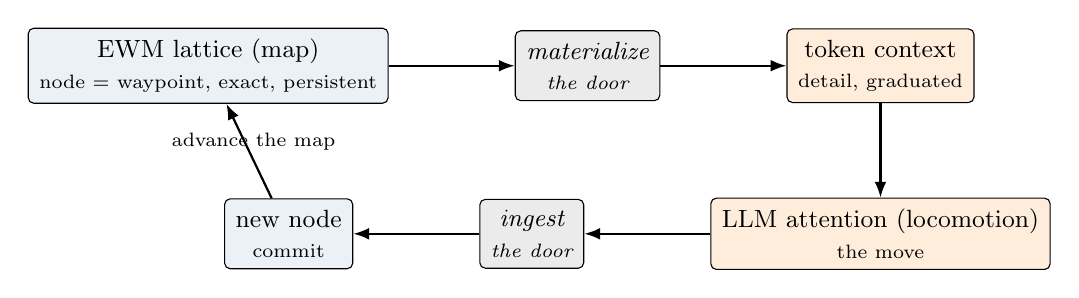
\begin{tikzpicture}[
  node distance=7mm,
  box/.style={draw, rounded corners=2pt, align=center, inner sep=4pt, font=\small},
  map/.style={box, fill=hlblue!8},
  tok/.style={box, fill=orange!14},
  door/.style={box, fill=black!8, font=\small\itshape},
  arr/.style={-{Latex[length=2mm]}, thick}
]
\node[map] (map) {EWM lattice (map)\\ \scriptsize node = waypoint, exact, persistent};
\node[door, right=16mm of map] (mat) {materialize\\ \scriptsize the door};
\node[tok, right=16mm of mat] (tok) {token context\\ \scriptsize detail, graduated};
\node[tok, below=12mm of tok] (move) {LLM attention (locomotion)\\ \scriptsize the move};
\node[door, left=16mm of move] (ing) {ingest\\ \scriptsize the door};
\node[map, left=16mm of ing] (new) {new node\\ \scriptsize commit};
\draw[arr] (map) -- (mat);
\draw[arr] (mat) -- (tok);
\draw[arr] (tok) -- (move);
\draw[arr] (move) -- (ing);
\draw[arr] (ing) -- (new);
\draw[arr] (new) -- node[above,font=\scriptsize,pos=0.4]{advance the map} (map);
\end{tikzpicture}
\caption{The travel loop. The lattice (map) names the waypoint; materialization
(door) restores the node's HLLSet context into token context; attention
(locomotion) makes the move inside that detail; ingestion (door, reverse)
re-compresses the result into a new node; the commit advances the map. The
support--union lemma is the exact seam between the map and the motion.}
\label{fig:loop}
\end{figure}

\subsection{The win-win}

\begin{table}[t]
\centering
\small
\renewcommand{\arraystretch}{1.15}
\begin{tabular}{@{}p{0.16\textwidth}p{0.37\textwidth}p{0.37\textwidth}@{}}
\toprule
 & \textbf{Lattice (the map)} & \textbf{Attention (the locomotion)} \\
\midrule
gives & exact waypoints; durable, auditable memory; controlled shrink/expand; collision groups & differentiable travel; detail resolution; generation of the next step \\
needs & a motor & a map \\
horizon & long, discrete, content-addressed & local, continuous, contextual \\
state & bitmap $S\subseteq\Plane$ (monotone) & convex coordinates $\xx\in\mathbb{R}^{d}$ (reversible) \\
failure mode & collision ambiguity at scale & context blow-up; drift; no durable state \\
\bottomrule
\end{tabular}
\caption{The win-win. Neither layer subsumes the other: the map has no motor
and the motor has no map, and materialization is the door that lets each hand
work to the other.}
\label{tab:winwin}
\end{table}

The table is the argument in miniature. A pure lattice engine can plan exactly
but cannot generate; a pure attention model can generate fluently but has no
exact, persistent notion of where it is and no bounded-cost way to hold a long
history. Joined at the seam, the lattice supplies the durability and the
address, and attention supplies the smooth motion and the detail. The
integration is not a replacement of either paradigm; it is the closure of both.

% ============================================================================
\section{The structural dictionary}
\label{sec:dictionary}
% ============================================================================

The correspondence theorem covers one attention head. A transformer is a
\emph{stack} of such heads with several architectural devices around them, and
each device has a counterpart in the EWM corpus. This section gives the
dictionary (Table~\ref{tab:dictionary}) and the propositions behind its rows.

\subsection{Multi-head attention is a family of worlds}

\begin{proposition}[Heads are worlds]
\label{prop:heads}
Let head $j$ use score $\sigm^{(j)}$ and values $V^{(j)}$. If each score factors
through an overlap form under a hash/seed configuration $\World_j=(h_j,s_j)$,
then the multi-head block is the holographic presentation of the world family
$\Omega=\{\World_j\}$: every head reads the \emph{same} lattice $\Lat$, and the
heads differ only in their interpretation fibres. The output projection $W_O$
is the bridge $\Bnd_{\Omega\to\World_0}$ of \eqref{eq:bridge} from the head
worlds back to the residual world $\World_0$.
\end{proposition}

\begin{proof}[Proof sketch]
By construction the head configurations are a finite set of hash configurations
with distinct scores. The companion note proves that a family of worlds over one
lattice is a fibred set $\mathcal{E}(\Omega)=\biguplus_{\World\in\Omega}
(\mathcal{N}_\tau(\World),\iotaw)$ whose base geometry is the shared lattice and
whose fibres are the interpretations \cite{companion2026}. Concatenating head
outputs is taking the total space; projecting by $W_O$ is the materialise--
transcribe--ingest composition that carries one world's reading into another,
i.e.\ the bridge. Determinism, idempotence on builders, and monotonicity are
Theorem~3 of the companion note.
\end{proof}

Proposition~\ref{prop:heads} explains two otherwise puzzling facts. First, the
heads \emph{share a representation but not a reading}: they can be edited
independently, and the companion note's \emph{virtual isolation} is exactly the
head-independence that makes multi-head attention work. Second, the output
projection is not a learned mixer over unrelated vectors; it is a
\emph{bridge}, and its job is to re-encode the head worlds into the residual
world. The empirical finding of the side-car project---``the only model-specific
code is a tiny adapter'' \cite{companion2026}---is the engineering face of the
same statement.

\subsection{Depth is complement traversal with a Noether stop}

\begin{proposition}[Depth and the stop criterion]
\label{prop:depth}
Let $M_0\supseteq M_1\supseteq\cdots$ be the sequence of merged nodes at
increasing traversal depth, let $C$ be the accumulated context, and let
$\Delta_d=M_d\setminus C$ be the complement of what has already been read.
Then $\Delta_0\supseteq\Delta_1\supseteq\cdots$ and the traversal terminates
exactly when $\Delta_d\approx\varnothing$, which is the Noether convergence
condition of the EWM evolution law \cite{ewm2026}. Attention depth is this
stopping problem; a compute-adaptive layer that exits when the complement is
empty is the exact analogue of an early-exit attention policy.
\end{proposition}

\begin{proof}
$C$ only grows (join is monotone), so $M_d\setminus C$ only shrinks; a shrinking
family of finite sets is eventually constant, and the level at which it first
equals the empty set is the first depth at which no new bit can be added. This
is the union invariant's conservation statement in the traversal order.
\end{proof}

Proposition~\ref{prop:depth} is the design that the cortex roadmap calls
\emph{complement-based temporal attention}: read only the part of each level not
already accumulated, quantify it with one overlap computation against the merged
node, and stop when nothing new remains \cite{roadmap2026}. Its cost is one
lattice operation per level rather than one per node per level, and its
correctness is the union invariant.

\subsection{Causal masking is the monotone ring basis}

\begin{proposition}[Causality, positions, and rotating coordinates]
\label{prop:causal}
For a causal (prefix) run, let $B(t)$ be the monotone ring basis of the
committed originals up to step $t$. Then masked attention reads only nodes of
$\spanof{B(t)}$, and the change of basis $B(t{-}1)\to B(t)$ transports head
coordinates exactly by a GF(2) matrix $M$: a coordinate vector $a$ at $t{-}1$
becomes $aM$ at $t$. Positional information is the trajectory frame
$\varphi_D(X)=(\BSS(X,D_1),\dots,\BSS(X,D_m))$; relative position is the
rotation of $B(t)$.
\end{proposition}

\begin{proof}
Causal masking keeps exactly the committed prefix, whose closed span is the
ring's monotone span \cite{state2026}. Monotonicity gives
$\spanof{B(t{-}1)}\subseteq\spanof{B(t)}$, so every old basis element has unique
coordinates in the new basis and transports by the change-of-basis matrix
(Proposition~4 of the state-machine paper). The frame statement is the
definition of a reading; the ring's per-commit re-pivoting is the rotating
coordinate system, measured at $534$ re-pivotings over $100$ commits on the
synthetic clip.
\end{proof}

Causal attention is thus a traversal of the \emph{monotone basis}, and the
familiar ``attention with positions'' is a traversal decorated with a moving
frame. The state-machine paper's distinction between a monotone basis and a
bounded visibility window is exactly the distinction between a global and a
sliding-window attention, with the same trade the transformer makes.

\subsection{The KV cache is the commit DAG}

\begin{proposition}[Cache and safe replay]
\label{prop:kv}
The key--value cache of an attention layer is a committed, content-addressed
stack: a key is the content address of a node, a write is a commit, and the
running state is the tip. Because ingestion is idempotent and the join is
union, reprocessing an uncommitted turn after a crash yields the same node as
processing it once; recovery is a pop, not a rebuild.
\end{proposition}

\begin{proof}
The cache is a set of IICA nodes; a node's name is its digest, so writing it
twice is a no-op and concurrent writes converge by re-registration
\cite{companion2026}. The safe-replay principle then gives the stated
idempotence \cite{state2026}.
\end{proof}

This proposition is why a lattice engine does not merely \emph{approximate} the
KV cache---it \emph{is} one, with the additional property that the cache is
shareable, auditable, and exact. The state-machine paper's storage discipline
(store only originals and base HLLSets; keep compounds as provenance-stamped
views recomputed on read) is a cache policy for attention keys and values.

\subsection{The residual stream is the union invariant}

\begin{proposition}[Residual = accumulation; $D/R/N$ = the write set]
\label{prop:residual}
The residual update $\xx_{l+1}=\xx_l+\Attn_l(\xx_l)$ corresponds, at the
lattice level, to the monotone accumulation $S(t{+}1)=S(t)\cup \HLL_{t+1}$; the
$D/R/N$ decomposition \eqref{eq:drn} is the write/keep/drop reading of one
attention step; and the union invariant
$H_{\mathrm{sys}}(t)=\bigcup_i L_i(t)$ is the conservation law that the residual
stream reproduces.
\end{proposition}

\begin{proof}
By Lemma~\ref{lem:support} the attention term contributes exactly the join of
the attended nodes; adding that join to the running state is the monotone
accumulation. The $D/R/N$ identities are \eqref{eq:drn}; that the union of all
temporal layers is conserved is the EWM temporal union theorem
\cite{ewm2026}, which is path-independence of the join and hence of the residual
stream.
\end{proof}

The EWM reading sharpens an intuition about transformers: the residual stream is
not an arbitrary additive channel but a \emph{conserved} accumulation, and the
attention layer is the selector that decides which bits enter it. ``Learning is
redistribution of attention across the lattice, not accumulation of weight
updates'' \cite{ewm2026} is the same statement from the EWM side.

\subsection{Q/K/V projections are the bootstrap permutation}

\begin{proposition}[Ashby and the projection family]
\label{prop:bootstrap}
The Q/K/V projections and the multi-head split are a bootstrap permutation
family in the sense of the Ashby--Bootstrap correspondence: each projection is a
view of the same token stream, and the union of views closes the variety gap
between the token vocabulary and the lattice plane. The $n$-gram bootstrap and
the projection family are the same construction at different levels of the
stack.
\end{proposition}

\begin{proof}
The Ashby--Bootstrap principle states that mismatched cardinalities are resolved
by measurement multiplication rather than capacity reduction
\cite{ewm2026,ashby1952}. A projection $W$ produces one view $XW$; a head
family produces $h$ views; their concatenation is the bootstrapped measurement
$H_\Pi(S)=\bigoplus_j H(\pi_j(S))$ with the $\pi_j$ the projection-induced
re-orderings. The n-gram family is the special case where the views are
contiguity windows.
\end{proof}

\clearpage
\subsection{The dictionary}

\begin{table}[!ht]
\centering
\small
\renewcommand{\arraystretch}{1.15}
\begin{tabular}{@{}p{0.30\textwidth}p{0.62\textwidth}@{}}
\toprule
\textbf{Transformer} & \textbf{EWM lattice} \\
\midrule
query $Q$ & ingested query HLLSet $I(\text{query})$ \\
key $K_i$ & stored node / content address (\texttt{h:}$\langle$sha1$\rangle$) \\
value $V_i$ & materialised tokens $M(K_i\cap Q)$, or a value node \\
score $\q\!\cdot\!\k$ & overlap form $\langle x,y\rangle$ under a learned metric \\
softmax weights & free-energy minimiser; entropic relaxation of thresholding \\
attention threshold & world BSS threshold $\tau$ \\
attention output & convex coordinates inside the selected support \\
$\supp(\text{output})$ & traversal join $\Trv_\theta(Q)=\bigcup_{\sigm\ge\theta}V_i$ \\
multi-head & world family $\Omega$; shared lattice, separate LUTs \\
output projection $W_O$ & bridge $\Bnd_{\Omega\to\World_0}$ \\
depth $L$ & complement traversal $\Delta_d=M_d\setminus C$ \\
early exit & Noether stop: $\Delta_d\approx\varnothing$ \\
causal mask & monotone ring basis $\spanof{B(t)}$ \\
position / relative position & trajectory frame; rotating coordinates \\
KV cache & commit DAG / tip (\texttt{ewm-git}) \\
residual stream $\xx\!\leftarrow\!\xx+\Attn$ & union invariant $S\!\leftarrow\!S\cup\HLL$ \\
$D/R/N$ & departed / retained / new decomposition \\
Q/K/V projections & bootstrap permutation family (Ashby) \\
layer norm & renormalisation preserving the invariant \\
retrieval-augmented generation & Mode~B set-key traversal (\S\ref{sec:engine}) \\
flash-attention tiling & a traversal \emph{order} over the key set \\
\midrule
node (waypoint) & place with detail compressed inside (HLLSet + LUT + matrix) \\
materialize-to-prompt & the door: HLLSet context $\to$ token context (\S\ref{sec:map}) \\
context window & managed working set, unpacked from the node on demand \\
context shrink / expand & meet with query / cover; union / lower threshold (\S\ref{sec:map}) \\
continuation hint & lattice-side seed for the next move \cite{ctx2026} \\
\bottomrule
\end{tabular}
\caption{The dictionary. Each row is a bead of the EWM corpus threaded onto a
transformer primitive; the first block is the seam (correspondence theorem), the
middle block the architecture (propositions above), and the last block the
map--journey interface of \S\ref{sec:map}.}
\label{tab:dictionary}
\end{table}

\FloatBarrier

% ============================================================================
\section{The exact engine}
\label{sec:engine}
% ============================================================================

The correspondence is not only a reading; it is an implementation. The cortex
design notes \cite{kspace2026,luttransformer2026} already specify an attention
whose key side is lattice-native, and the three modes there are exactly the
points of the temperature axis of \S\ref{sec:bridge}. In the travel picture,
Mode~B is the map selecting the waypoint, Mode~A is locomotion over the
lattice's own key partition, and Mode~C is locomotion steered by the map.

\subsection{Three modes}

\begin{description}[leftmargin=*,style=nextline]
  \item[Mode A (address-key, tier 1).] A token's key is its bit address,
    $\k_t=E_{\mathrm{bit}}[\mathrm{bit}(t)]$, with $E_{\mathrm{bit}}$ a learned
    $32{,}768\times d$ table. Tokens in the same cell share a key; $V$ and
    context disambiguate within a cell. This is the \emph{relaxed} end: the
    lattice supplies the partition, learning supplies the metric. The pure
    hashing variant $\k_t=\text{one-hot}(\mathrm{bit}(t))W_K$ with $W_K$ fixed
    is Reformer-style bucketed attention \cite{kitaev2020}.
  \item[Mode B (set-key, tier 2/3).] The query and the keys are HLLSets,
    $Q_{\mathrm{hll}}=I(\text{prefix})$, $K_{\mathrm{hll}}=C$ (the context
    sub-lattice), the score is lattice containment $\BSS_\tau(Q_{\mathrm{hll}}
    \subseteq K_{\mathrm{hll}})$ or Jaccard, and the value is
    $M(K_{\mathrm{hll}}\cap Q_{\mathrm{hll}})$. This is the \emph{exact} end
    and corresponds to the \emph{map lookup} that picks the waypoint: no dot
    product over learned vectors, only a lattice morphism and LUT extraction. It
    is the HLLSet-native attention exercised by CAAL-LLM's
    \texttt{suggest\_continuations} routine, and it is the general form of which
    retrieval-augmented generation \cite{lewis2020} is a special case.
  \item[Mode C (hybrid).] $\sigm(i,j)=\q_i\!\cdot\!\k_j/\sqrt{d}
    +\lambda\,\varphi(Q_{\mathrm{hll}},K_{\mathrm{hll}})$, with $\varphi$ a
    lattice similarity and $\lambda$ learned or scheduled. The learned
    dot-product remains the workhorse; the lattice term steers it toward the
    selected waypoint, and the contribution is measurable by ablation
    ($\lambda=0$ versus $\lambda>0$).
\end{description}

The three modes are not three algorithms but three temperatures. Mode~A is
attention with a lattice-shaped key space; Mode~B is hard traversal, the map
lookup; Mode~C is a traversal-steered relaxation. Moving from C to B is exactly
lowering the temperature on the lattice term.

\subsection{Coverage is the exactness gauge}

The exact engine's correctness condition is the \emph{coverage invariant}:
the reverse index must cover the active bits of the managed sub-lattice,
\begin{equation}
\label{eq:coverage}
  \Lut.\mathrm{bits}\ \supseteq\ \mathrm{bits}(C),
  \qquad
  \mathrm{confidence}(C)=\frac{\text{resolved bits}}{\text{total bits}}=1.0 .
\end{equation}
Under coverage, the sub-lattice extraction $M(Q\cap C)$ is deterministic, touches
no bit outside $C$, and is exact up to governing tier: tier~1 exact up to
collision groups, tier~2 exact membership by multi-seed quorum, tier~3
disambiguated by $2$/$3$-gram structure and De Bruijn order
\cite{kspace2026}. The collision statistics are the resolution budget of the
key space: with the soldered geometry the pairwise collision probability is
$p=1/3072$, and a sub-vocabulary of $n$ active tokens carries
$\binom{n}{2}p$ expected collisions---near-exact for $n\lesssim 300$, and
repairable by a second and third seed at $p^2\approx10^{-7}$ and
$p^3\approx10^{-11}$ \cite{kspace2026}. This is the price list of the exact
end of the temperature axis, and it is the lattice's account of why a small
context---one node---can be routed and unpacked exactly.

\subsection{Traversal order: tiling and content addressing}

Attention is a \emph{set} operation, but it is computed in an \emph{order}, and
the order is where the systems work lives. FlashAttention \cite{dao2022}
computes exact softmax attention by tiling the key matrix and carrying an online
softmax normaliser, so that the operator is realised without materialising the
$n\times n$ matrix. In the dictionary this is a traversal order over the key
set: the keys are blocks, the running normaliser is the accumulator, and the
algorithm is exact because the join and the normaliser are associative.

The lattice engine's traversal order is different in kind. Because keys are
content-addressed, the key set is not a contiguous matrix but the commit DAG;
traversal follows the DAG from the tip, and the ring basis orders the nodes by
their pivots. The order is chosen for \emph{reachability} rather than for
memory locality, and the complement stop (\S\ref{sec:dictionary}) prunes it.
The two orders are complementary: flash-attention tiles a dense key set for
throughput; the lattice traverses a sparse, content-addressed key set for
exactness and replay. Both are traversals, and both are exact.

\subsection{Traversal signals are measurable}

The engine's readings are not hypothetical. On the state machine's synthetic
$10\times10$ scene clip the lattice traversal produces exactly the signals an
attention diagnostic would want \cite{state2026}: the linear residual detects
all nine scene cuts ($2.9\times$ separation for the windowed morphism), the bit
novelty $N=X\setminus\mathrm{cover}$ separates cuts from in-scene drift by
$3.75\times$, symmetric differences lie in the ring span in $394/394$ cases
while meets and joins do not, and the rotating-coordinate view re-pivots $534$
coordinates over $100$ commits with the pre-commit residual spiking at every
cut. In the dictionary these are the traversal's \emph{novelty}, \emph{surprise},
\emph{representability}, and \emph{re-basing} signals; they are the lattice's
account of what a move is doing when it is doing something interesting, and
they are the natural triggers for opening the door of \S\ref{sec:map}.

% ============================================================================
\section{Why the pair is all you need}
\label{sec:all}
% ============================================================================

The title is a claim about primitives, and in the two-layer reading it is a
claim about a \emph{pair}. ``Attention on lattice traversal'' names the
composite: the map (lattice traversal), the motion (attention), and the door
(materialization) that joins them. The claim is that this composite is
complete---and that neither half is.

\paragraph{The map has no motor; the motor has no map.}
This is the whole argument, and Table~\ref{tab:winwin} states it. A lattice
engine can decide exactly \emph{where} to go, hold a long history at a bounded
cost, and prove that a recomputation is safe; it cannot generate fluent detail
or resolve the meaning of a collision without unpacking the node. An attention
model can generate fluently and move smoothly through detail; it has no exact,
persistent notion of where it is, and its context grows with everything it has
seen. Each layer is precisely what the other lacks. The seam
(Lemma~\ref{lem:support}, Theorem~\ref{thm:correspondence}) is what makes the
join lossless, and the door (the round-trip law, \S\ref{sec:map}) is what makes
it safe to cross repeatedly.

\paragraph{Sufficiency of the pair.} A composite of the map and the motion
supplies each of the five functional properties of attention
(Section~\ref{sec:attn}):
\begin{center}
\small
\begin{tabular}{@{}ll@{}}
\toprule
\textbf{Attention property} & \textbf{Supplied by} \\
\midrule
content routing & lattice traversal: $\sigm$ is a function of $Q,K_i$ alone (Def.~\ref{def:traversal}) \\
permutation equivariance & $\sigm$ and the join are order-independent (Thm~\ref{thm:correspondence}(4)) \\
competition & the free energy normalises the weights (Thm~\ref{thm:free}) \\
value aggregation & the join accumulates values (Lemma~\ref{lem:support}) \\
composability & IICA composition; the union invariant (Props~\ref{prop:depth}--\ref{prop:residual}) \\
\emph{detail} & materialization: the node's compressed context unpacked to tokens (\S\ref{sec:map}) \\
\bottomrule
\end{tabular}
\end{center}
The first five rows are the seam; the last row is the job attention does that
the map alone cannot, and it is the reason the pair, not the traversal alone, is
the primitive.

\paragraph{Necessity.} Conversely, any operator that routes by a query--key
similarity and aggregates values is an instance of Definition~\ref{def:traversal}
with $\theta$ equal to its selection rule and $\tau$ its temperature
(Theorem~\ref{thm:free}); and any bounded-context generator that must persist
state across sessions needs the map, because the token context is transient by
construction. So the pair is not a choice between two designs; it is the
minimal closure of either one.

\paragraph{What the integration buys, concretely.}
\begin{itemize}[leftmargin=*,nosep]
  \item \textbf{Unbounded, auditable memory at bounded cost.} A node is $4$\,KB
    packed; the map holds a long history as content-addressed nodes, and the
    trajectory is replayable \cite{state2026,companion2026}.
  \item \textbf{Attention that runs where it matters.} Attention is applied to
    the selected node's context, not to the whole history; the map prunes the
    key set before the motion begins.
  \item \textbf{Exactness with a measurable budget.} The waypoint is
    content-addressed and the door round-trips; collisions are the only
    inexactness, and they are quantified \cite{kspace2026}.
  \item \textbf{Controllable context.} Shrink and expand the node with lattice
    operations before materialising, so the working set is a design choice, not
    a by-product of sequence length \cite{ctx2026}.
\end{itemize}

\paragraph{The seam, once more.} In attention, the state is the convex
coordinate vector $\xx\in\mathbb{R}^{d}$; selection is soft and reversible, and
the support is emergent. In the lattice, the state is the bitmap
$S\subseteq\Plane$; selection is hard and monotone, and the coordinates are the
emergent, basis-relative reading. Lemma~\ref{lem:support} is the bridge between
them: support maps one to the other, and the free energy is the interpolation
along the way. ``Attention on lattice traversal is all you need'' therefore has
a literal operational meaning: draw the map, walk it with attention, and cross
through materialization---the rest is temperature.

% ============================================================================
\section{Related work}
\label{sec:related}
% ============================================================================

\paragraph{Attention.} The mechanism is from \cite{vaswani2017}, with the
query--key--value reading rooted in additive attention \cite{bahdanau2015}. The
retrieval reading is developed by \cite{ramsauer2020}, which shows that
transformer attention is the update rule of a modern Hopfield network and hence
an associative-memory retrieval; our support--union lemma is the lattice-side
counterpart of that identification, and it makes the retrieval exact at zero
temperature. Efficient attention by hashing and kernels
\cite{kitaev2020,choromanski2021} trades exactness for sub-quadratic cost by
\emph{changing the key partition}---precisely the K-representation choice that
the partition principle of \cite{kspace2026} says is free. FlashAttention
\cite{dao2022} is the traversal-order result discussed in \S\ref{sec:engine}.
Retrieval-augmented generation \cite{lewis2020} is Mode~B, the map lookup.

\paragraph{World models and memory.} World models learn a predictive latent
state \cite{ha2018}; JEPA-style architectures separate encoder, context, and
predictor \cite{lecun2022}. EWM differs by making the state
\emph{content-addressed} and the transitions \emph{lattice operations}, and the
state-machine paper shows the resulting state layer is a side-car that any
model can attach \cite{state2026}; the context design shows the same layer can
\emph{generate the prompt} from the stored HLLSet state \cite{ctx2026}. The
uncertainty-reduction appendix of the main EWM paper \cite{ewm2026,lincoln2026}
reads the traversal's novelty signal as a content-blind primary reinforcer,
which is the reward-side analogue of the locomotion story here.

\paragraph{Sketches and content-addressed storage.} HLLSets descend from
probabilistic cardinality estimation \cite{flajolet2007} and resemblance
sketches \cite{broder1997,bloom1970}, but are used here as \emph{state}, not as
estimators. Content addressing underlies Merkle trees \cite{merkle1988},
Git \cite{git}, and IPFS/IPLD \cite{benet2014}; the lattice's joins are the
CRDT-style merge of \cite{shapiro2011}. The EWM main paper's
Grothendieck-topology target \cite{grothendieck1972} and the companion's
geometric-morphism reading of bridges make the world family a site; the
correspondence theorem is the finite, explicit stage of that programme.

\paragraph{The originals.} The four EWM principles \cite{ewm2026}, the lattice
and its worlds \cite{companion2026}, the state machine and its trajectory
\cite{state2026}, the HLLSet algebra \cite{astesj2026}, and the design notes on
HLLSet K-space, the LUT transformer, temporal attention, the cortex, and the
conversation context
\cite{kspace2026,luttransformer2026,roadmap2026,cortex2026,ctx2026} are the
beads this paper threads. The Boolean-lattice background is \cite{birkhoff1940};
the variety law is \cite{ashby1952}; the conservation-law reading is
\cite{noether1918}.

% ============================================================================
\section{Discussion and limitations}
\label{sec:discussion}
% ============================================================================

\paragraph{The seam is structural, not numerical.} We have shown that the two
layers share a support operator and a similarity geometry. We have
\emph{not} shown that a given trained transformer's weights equal a given
lattice traversal's scores; the correspondence is at the level of the operator,
and the learned metric remains learned. The dictionary is an identification of
roles, and its value is explanatory and constructive, not an equivalence of
trained parameters.

\paragraph{The door is faithful, not lossless in content.} The round-trip law
recovers the 1-HLLSet exactly and the structural layers up to collision
ambiguity \cite{ctx2026}. Materialization returns the builders plus any
collision neighbours; the door preserves the sketch, not the original text. A
traveller who needs the exact prose must keep it as an original node, not as a
derived one---which is exactly the state machine's storage discipline.

\paragraph{Soft support is total.} Because softmax is strictly positive, an
untruncated attention row has full support; Lemma~\ref{lem:support} then says
its bitmap is the join of \emph{all} context values. This is a feature, not a
paradox: it is why the residual stream accumulates broadly while the weights
carry the motion. The hard traversal is the truncated case, and the truncation
is the threshold that EWM makes explicit. An untruncated attention layer is a
traversal at positive temperature with $\theta=-\infty$.

\paragraph{Exactness has a resolution budget.} The lattice's exact end pays in
collisions ($p=1/3072$ per pair) and in materialisation ambiguity. The engine
manages it with a multi-seed quorum, structural layers, and the coverage
invariant, but the budget is real; a large active node requires the higher
tiers, and the tiers cost computation. The dense end pays instead in quadratic
compute and inexact retrieval. The temperature axis is also a cost axis.

\paragraph{The ring is linear; attention is not.} The ring's span is a GF(2)
subspace, closed under symmetric difference but not under intersection, union,
or difference; the meet is the obstruction, and the residual is the exact
distance of a node from the context span \cite{state2026}. Attention's softmax
is nonlinear in a different way. The dictionary identifies the ring with the
causal prefix, but the two nonlinearities are not the same map, and translating
a trajectory reading into a locomotion diagnostic (and back) is an open
problem.

\paragraph{Open questions.} (1) Does the map/motion reading suggest a
controller that opens the door only when a traversal signal fires---a
\emph{surprise-gated} materialization policy? (2) Can the exact engine's
threshold be made differentiable without losing the bitmap (a soft support with
hard bits)? (3) Is there a canonical waypoint-selection policy over the commit
DAG analogous to flash-attention's tiling? (4) The companion note's bridges are
geometric morphisms only in the order-theoretic sense; the full sheaf condition
on the world site is still the EWM programme's open target, and the map/motion
reading inherits that openness.

% ============================================================================
\section{Conclusion}
\label{sec:conclusion}
% ============================================================================

The EWM lattice is the map: a coarse, exact, persistent, content-addressed graph
of places, each node a compact HLLSet that carries its detail compressed inside.
Attention is the locomotion: the fine, graduated, differentiable mechanism that
moves the model once a node's detail has been unpacked. Materialization is the
door between them: it restores HLLSet context to token context, and ingestion
takes the result back to the map. The seam is one lemma---the support of an
attention layer is the lattice join of the value nodes it attends to---so the
bitmap fixes the working set and the weights make the move; and the softmax is
the entropic relaxation of the traversal threshold, so temperature and threshold
are two faces of one knob. Around the seam every transformer device falls into
place: heads are worlds, the output projection is the bridge, depth is
complement traversal with a Noether stop, causality is the monotone ring basis,
positions are rotating coordinates, the KV cache is the commit DAG, the residual
stream is the union invariant with its $D/R/N$ reading, and Q/K/V are the
bootstrap permutation.

The two paradigms are not rivals and not the same: they are the two halves of
one journey, and ``attention on lattice traversal'' is the complete primitive.
The map has no motor, the motor has no map, and the door is what lets each hand
work to the other.

The Glass Bead Game is won by the move that makes the board legible. The move
here is to see that the beads were never rivals---one set drew the map, another
walked it, and the game is the journey.

% ============================================================================
\section*{Acknowledgment}
% ============================================================================
This article was written in collaboration between the authors and an AI
assistant, following the practice of the companion and state-machine papers.
The human authors developed the EWM framework, the HLLSet algebra, and the
\texttt{ewm-state-machine} realisation, and directed the line of argument; the
AI assistant helped to draft and structure the text, work through the formal
statements, and thread the correspondence with the existing corpus. The
conceptual content is the authors' own.

% ============================================================================
\appendix
\section{Notation}
% ============================================================================

\begin{center}
\small
\begin{tabular}{@{}ll@{}}
\toprule
\textbf{Symbol} & \textbf{Meaning} \\
\midrule
$\Plane=\{0,\dots,\Reg\Bits-1\}$ & bit plane ($32{,}768$ positions at defaults) \\
$\Lat=(2^{\Plane},\subseteq,\cup,\cap,\xor)$ & EWM Boolean lattice (the map) \\
$\LatR=\mathbb{R}^{\Plane}$ & realification; the hypercube's ambient space \\
$\HLL(A)$ & HLLSet of token collection $A$ (a waypoint's coordinate) \\
$\mu$, $\mu_\World$ & measurement morphism (IICA) \\
$\World=(h,s,\tau)$ & world: hash type, seed, BSS threshold \\
$\Lut_\World$, $\iotaw$ & world LUT and interpretation \\
$\Bnd_{\World_1\to\World_2}$ & bridge (ingest $\circ$ transcribe $\circ$ materialise) \\
$\BSS_\World(X)=|X\cap B_\World|/|B_\World|$ & BSS against the world basis \\
$H(t)=(S(t),H(t{-}1),D,R,N)$ & state equation \eqref{eq:fundamental} \\
$\Ctx_{\mathrm{tok}}$ & token context (the materialised working set) \\
$\mathrm{materialize}/\mathrm{ingest}$ & the door between lattice and token context \\
$\sigm(Q,K)$ & traversal score \\
$\tau$, $\theta$ & temperature, threshold \\
$\Trv_\theta(Q)=\bigcup_{\sigm\ge\theta}V_i$ & thresholded traversal join \\
$\Attn_\theta$ & truncated attention operator \\
$\supp(\cdot)$ & set of non-zero coordinates \\
$\spanof{B}$ & GF(2) span of the ring basis $B$ \\
$\res(X)$ & residual of $X$ against the span \\
\bottomrule
\end{tabular}
\end{center}

% ============================================================================
\section{Proofs}
\label{app:proofs}
% ============================================================================

\paragraph{Lemma~\ref{lem:overlap} (overlap is a bilinear form).} Already proved
in place. The identities follow by counting $b$ with $x_by_b=1$.

\paragraph{Lemma~\ref{lem:support} (support--union).} Already proved in place.
The only used facts are $\alpha_i\ge0$ and $V_{i,b}\in\{0,1\}$; the result fails
if weights may be negative, which is exactly the cancellation that the lattice
forbids and the convex stream permits.

\paragraph{Theorem~\ref{thm:free} (free energy).} The Lagrangian computation is
in place. Two standard consequences are used: (i) the Gibbs distribution is the
unique minimiser because $F_\tau$ is strictly convex on the simplex for $\tau>0$;
(ii) the low-temperature limit concentrates on the argmax and the
high-temperature limit on the uniform distribution.

\paragraph{Theorem~\ref{thm:correspondence}.} (1) Lemma~\ref{lem:support}.
(2) Theorem~\ref{thm:free}. (3) The support of the truncated Gibbs distribution
is constant in $\tau$ for $\tau>0$ and equal to the $\theta$-superlevel set; as
$\tau\to0$ the untruncated weights concentrate on the argmax, and the
corresponding join is the join of the argmax set by finiteness of
$\mathcal{K}$. (4) Relabel the keys by a permutation $\pi$; then
$\sigm(Q,K_{\pi(i)})=\sigm(Q,K_i)$ as a multiset and
$\bigcup_i V_{\pi(i)}=\bigcup_i V_i$ because union is commutative and
idempotent.

\paragraph{Proposition~\ref{prop:heads}.} Invoke the companion note's
world-family theorem and bridge theorem; the concatenation is the total space
$\mathcal{E}(\Omega)$ and the projection is the bridge composition
\eqref{eq:bridge}. Monotonicity of the bridge gives that increasing the head
set can only add support to the residual world.

\paragraph{Proposition~\ref{prop:residual}.} Lemma~\ref{lem:support} gives the
support identity; $D/R/N$ is \eqref{eq:drn}; the union invariant is the main
paper's temporal union theorem. Path-independence of the join is the reason the
residual stream is order-independent, which is the conservation statement.

\paragraph{Round-trip law (\S\ref{sec:map}).} The 1-HLLSet direction is exact
because materialization emits only tokens whose 1-gram bits are set in the
source and ingestion is a union over those tokens, so no bit outside the source
1-HLLSet can be added and no set bit can be missed; the structural layers are
exact when the LUT covers the builders and otherwise exact up to
collision-induced extra paths that must survive both shape filtering and the
1-/2-gram cross-validation \cite{ctx2026}.

% ============================================================================
\section{Implementation map}
% ============================================================================

\begin{table}[h]
\centering
\small
\begin{tabular}{@{}p{0.34\textwidth}p{0.58\textwidth}@{}}
\toprule
Concept & Artifact \\
\midrule
bit plane, HLLSet & \texttt{hllset\_core::HLLSet} (Roaring bitmap) \\
geometry $\Prec,\Reg,\Bits$ & \texttt{hllset\_contracts} ($P$, $M$, \texttt{BITS\_PER\_REG}) \\
morphism $\mu$ & \texttt{hllset\_morphisms::ingest / materialize} \\
working state $S(t)$ & \texttt{ewm-app::StateCache::working} \\
base $H(t{-}1)$ & commit tip (\texttt{ewm-git}) \\
$D/R/N$ & \texttt{ewm-scene::noether} and the commit decomposition \\
ring basis, push & \texttt{ewm-boolring::BoolWindow} \\
commit DAG, tip & \texttt{ewm-git} (\texttt{commit}, \texttt{head}) \\
trajectory frame, soft key & \texttt{context-tree}, ring projections \\
world, bridge & hash configuration $(h,s)$; two-pass side-car loop \\
the door & \texttt{hllset-context::to\_prompt / restore} (\S\ref{sec:map}) \\
context shrink / expand & sub-lattice restriction, cover, union, threshold \\
K-storage interface & \texttt{hllset-attn::KStorage} (\texttt{key\_of}, \texttt{candidates}, \texttt{confidence}) \\
Mode A key table & \texttt{hllset-attn::bit\_table} ($E_{\mathrm{bit}}$) \\
Mode B/C scores & \texttt{hllset-attn::setkey / hybrid} (BSS, Jaccard, $\lambda$) \\
\bottomrule
\end{tabular}
\caption{Concept-to-code correspondence, extending the state-machine paper's
map with the attention crates proposed in the cortex design notes
\cite{kspace2026,luttransformer2026} and the door of the context design
\cite{ctx2026}.}
\label{tab:impl}
\end{table}

% ============================================================================
\begin{thebibliography}{99}

\bibitem{ewm2026} A.~Mylnikov, A.~Mylnikov Jr., and D.~Kumar,
\textit{Emerging World Models: A Structural Framework for Self-Organizing World
Representations}, 2026. (First paper of the EWM series; four foundation
principles.)

\bibitem{companion2026} A.~Mylnikov, A.~Mylnikov Jr., and D.~Kumar,
\textit{The EWM Lattice and Its Worlds: HLLSets, Emerging Lattices, and
Multi-World Representation}, companion note to \textit{Emerging World Models},
2026.

\bibitem{state2026} A.~Mylnikov, A.~Mylnikov Jr., and D.~Kumar,
\textit{Transformations and Trajectories of a Content-Addressed State Machine:
The Emerging World Model HLLSet Architecture}, 2026. (TECS submission draft.)

\bibitem{astesj2026} A.~Mylnikov,
\textit{HLLSet Theory: A Unified Framework for Probabilistic Knowledge
Representation}, ASTESJ, Vol.~11, No.~2, pp.~62--74, 2026.
\url{https://www.astesj.com/publications/ASTESJ_110202.pdf}

\bibitem{kspace2026} A.~Mylnikov,
\textit{HLLSet as the K-Space of Attention: Mathematical Summary}, cortex
design note, \texttt{ewm-cortex/docs/HLLSET\_K\_SPACE\_MATH.md}, 2026.

\bibitem{luttransformer2026} A.~Mylnikov,
\textit{Reproduction Transformer with HLLSet LUT-based K-Storage:
Architecture}, cortex design note,
\texttt{ewm-cortex/docs/HLLSET\_LUT\_TRANSFORMER\_ARCHITECTURE.md}, 2026.

\bibitem{roadmap2026} A.~Mylnikov,
\textit{HLLSet Transformer Architecture: Temporal Attention via W Lattice
Backpropagation}, design roadmap,
\texttt{hllset\_algebra/DOCS/HLLSET\_TRANSFORMER\_ROADMAP.md}, 2026.

\bibitem{cortex2026} A.~Mylnikov,
\textit{ewm-cortex: Enhanced HLLSet Cortex Architecture}, 2026.

\bibitem{ctx2026} A.~Mylnikov,
\textit{Conversation Context over HLLSet --- Design}, context design note,
\texttt{hllset-next/\_DOCS/arch/CONVERSATION\_CONTEXT\_LLM.md}, 2026.
(Materialize-to-prompt and the round-trip composition law.)

\bibitem{vaswani2017} A.~Vaswani, N.~Shazeer, N.~Parmar, J.~Uszkoreit,
L.~Jones, A.~N.~Gomez, \L.~Kaiser, and I.~Polosukhin,
\textit{Attention Is All You Need}, NeurIPS, 2017.

\bibitem{bahdanau2015} D.~Bahdanau, K.~Cho, and Y.~Bengio,
\textit{Neural Machine Translation by Jointly Learning to Align and Translate},
ICLR, 2015.

\bibitem{kitaev2020} N.~Kitaev, \L.~Kaiser, and A.~Levskaya,
\textit{Reformer: The Efficient Transformer}, ICLR, 2020.

\bibitem{choromanski2021} K.~Choromanski et al.,
\textit{Rethinking Attention with Performers}, ICLR, 2021.

\bibitem{dao2022} T.~Dao, D.~Y.~Fu, S.~Ermon, A.~Rudra, and C.~R\'e,
\textit{FlashAttention: Fast and Memory-Efficient Exact Attention with
IO-Awareness}, NeurIPS, 2022.

\bibitem{ramsauer2020} H.~Ramsauer et al.,
\textit{Hopfield Networks Is All You Need}, ICLR, 2021.

\bibitem{lewis2020} P.~Lewis et al.,
\textit{Retrieval-Augmented Generation for Knowledge-Intensive NLP Tasks},
NeurIPS, 2020.

\bibitem{lecun2022} Y.~LeCun,
\textit{A Path Towards Autonomous Machine Intelligence}, 2022.

\bibitem{ha2018} D.~Ha and J.~Schmidhuber,
\textit{World Models}, arXiv:1803.10122, 2018.

\bibitem{flajolet2007} P.~Flajolet, \'E.~Fusy, O.~Gandouet, and F.~Meunier,
\textit{HyperLogLog: The Analysis of a Near-Optimal Cardinality Estimation
Algorithm}, AofA, 2007.

\bibitem{bloom1970} B.~H.~Bloom,
\textit{Space/Time Trade-offs in Hash Coding with Allowable Errors},
Comm.\ ACM, 13(7):422--426, 1970.

\bibitem{broder1997} A.~Z.~Broder,
\textit{On the Resemblance and Containment of Documents}, Compression and
Complexity, 1997.

\bibitem{murmur3} A.~Appleby,
\textit{MurmurHash3}, 2011. x64-128 variant; the seed is a parameter of the
measurement.

\bibitem{merkle1988} R.~C.~Merkle,
\textit{A Digital Signature Based on a Conventional Encryption Function},
CRYPTO, 1987.

\bibitem{git} S.~Chacon and B.~Straub,
\textit{Pro Git}, Apress, 2nd ed., 2014.

\bibitem{benet2014} J.~Benet,
\textit{IPFS---Content Addressed, Versioned, P2P File System},
arXiv:1407.3561, 2014.

\bibitem{shapiro2011} M.~Shapiro, N.~Pregui\c{c}a, C.~Baquero, and
M.~Zawirski,
\textit{Conflict-Free Replicated Data Types}, SSS, 2011.

\bibitem{birkhoff1940} G.~Birkhoff,
\textit{Lattice Theory}, American Mathematical Society, 1940.

\bibitem{ashby1952} W.~R.~Ashby,
\textit{Design for a Brain}, Chapman \& Hall, 1952.

\bibitem{noether1918} E.~Noether,
\textit{Invariante Variationsprobleme}, Nachr.\ d.\ K\"onig.\ Gesellsch.\ d.\
Wiss.\ zu G\"ottingen, Math-phys.\ Klasse, pp.~235--257, 1918.

\bibitem{grothendieck1972} A.~Grothendieck et al.,
\textit{Th\'eorie des topos et cohomologie \'etale des sch\'emas (SGA 4)},
Springer LNM 269, 1972.

\bibitem{lincoln2026} C.~Lincoln,
\textit{Uncertainty Reduction as a Primary Reinforcer}, 2026. (Cited in the
EWM main paper's reinforcement appendix.)

\bibitem{hess1943} H.~Hesse,
\textit{Das Glasperlenspiel (The Glass Bead Game)}, Fretz \& Wasmuth, 1943.

\end{thebibliography}

\end{document}
